\documentclass{article}
\usepackage{graphicx}
\usepackage[section]{placeins}
\usepackage[a4paper,margin=0.75in]{geometry}
\usepackage{array}
\usepackage{varwidth}
\usepackage{tabularx}
\usepackage{amsmath}
\usepackage{subcaption}

\graphicspath{{../plots/}}

\title{COL380 Assignment 1 report}
\title{LU Decomposition using Pthreads and OpenMP}
% \author{Brian Sajeev Kattikat \\ {2021CS50609}}
\date{February 2024}

\begin{document}

\maketitle

\section{Code overview}
\subsection{Pthreads}

\subsection{OpenMP}

\section{Design decisions}

\subsection{Pthreads}

\subsection{OpenMP}


\section{Runtime Analysis}

Following are the obtained plots for Parallel efficiency vs number of threads

% \begin{figure}[!htb]
%     \centering
%     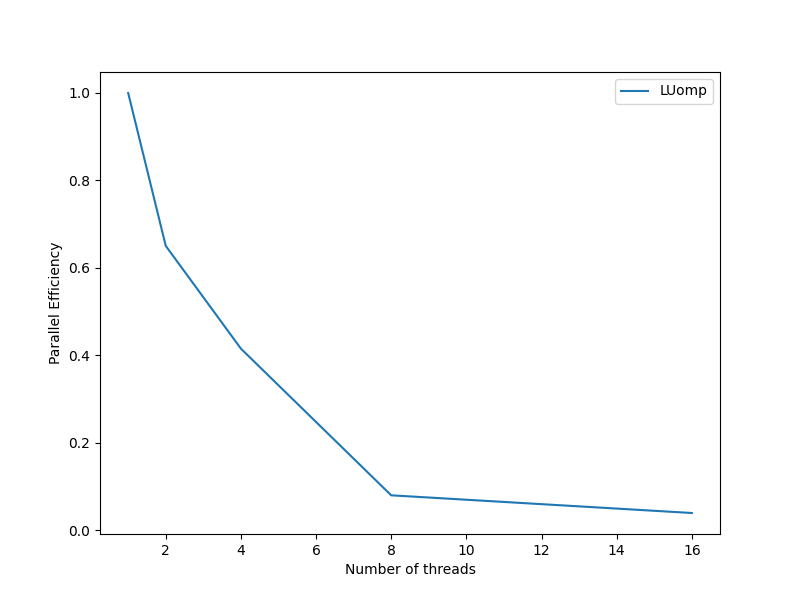
\includegraphics[width=13cm]{LUomp.png}
%     \caption{OpenMP}
%     % \label{fig:1}
% \end{figure}
%
% \begin{figure}[!htb]
%     \centering
%     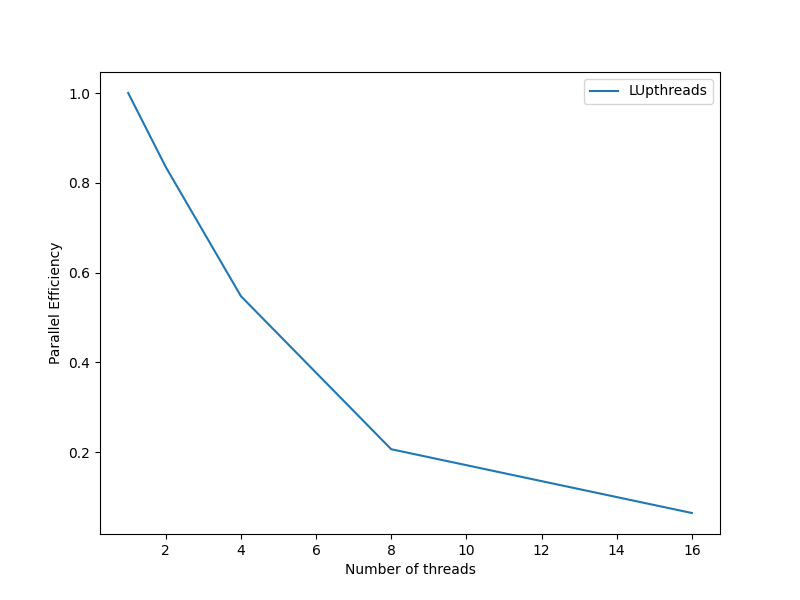
\includegraphics[width=13cm]{LUpthreads.png}
%     \caption{Pthreads}
%     % \label{fig:1}
% \end{figure}

\begin{figure}[!htb]
    \centering
    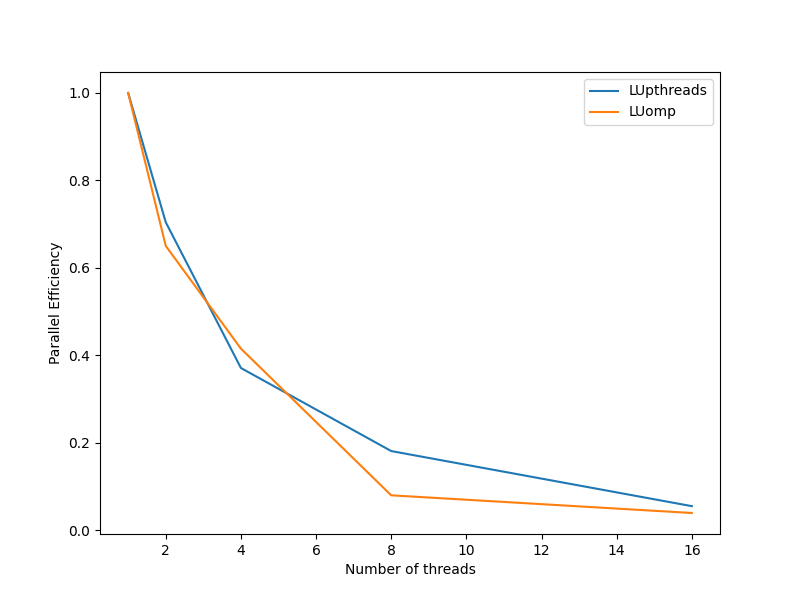
\includegraphics[width=13cm]{Both.png}
    \caption{Both OpenMP and Pthreads}
    % \label{fig:1}
\end{figure}

\end{document}
